\documentclass[twocolumn,11pt]{article}
\usepackage{authblk}
\usepackage{graphicx}
\usepackage{hyperref}
\usepackage{amsmath}
\usepackage{lipsum,adjustbox}
\usepackage{tikz}
\usetikzlibrary{calc, positioning}


\title{Tor Inter-Relay Latency}
\author[1]{Frank Cangialosi}
\author[1]{Scott DellaTorre}
\author[1]{Emily Kowalczyk}
\author[1]{Brent Schlotfeldt}
\author[1]{Dave Levin\thanks{Faculty Advisor}}
\affil[1]{University of Maryland}
\date{}
\raggedbottom

\begin{document}
\maketitle

\section {Introduction}

The Internet, once a small network of hosts operated primarily by large academic and governmental institutions, has grown dramatically in the decades since its conception. The result, an exceedingly complex network comprised of billions of intercommunicating hosts, is much more difficult to analyze than the system from which it evolved. At the same time, the importance of such analysis is perhaps greater now than it ever was. Millions of people have become daily users of the Internet, relying on the network to quickly access information and communicate with their peers. Less frequent users number in the billions, and thousands more gain Internet access every day. As network designers, engineers, and researchers strive to accommodate the ever-increasing demands of these and future users, their success will depend in part on their ability to determine the current state of the network. Indeed, the designers of the future Internet will need to recognize and address problems that the network currently faces, and be able to adapt their solutions in response to changing network conditions. In pursuit of these goals, their access to comprehensive and up-to-date network statistics will be essential.
	
Unfortunately, gathering this information on a large scale is difficult. Although there exist many tools to measure network statistics, they require direct access to a source host. For example, \texttt{ping} and \texttt{traceroute}--networking utilities which provide useful information such as network latency, packet loss, and the route taken by packets--do so by sending small data packets from an originating host to a destination host. Thus, tools such as these can only generate measurements that originate from a controlled source. This requirement hinders the ability of  researchers to compute comprehensive network statistics. Indeed, a researcher is limited both by the number of host machines to which he or she has access and the locations of these hosts. Using existing tools, a researcher cannot choose two arbitrary hosts, or even two arbitrary locations, and determine the network conditions between them. If we could provide researchers this ability, it would greatly expand their access to global network conditions, allowing them to produce much more comprehensive analyses of the global Internet than are currently possible.

Of course, access to arbitrary hosts on the Internet is not a feasible goal. This would require every user to volunteer a portion of their network bandwidth to research, a contribution only a small fraction of users would likely be willing to make. Nevertheless, by tapping into this collection of volunteered hosts, we can achieve a much more refined picture of the global Internet. Researchers have used this strategy in past studies, taking network measurements using hosts volunteered to PlanetLab, a group of computers available as a testbed for computer networking and distributed systems research, and other public clusters \cite{PlanetLab}. However, the vast majority of hosts in such clusters are administered by large corporations and academic institutions. These organizations connect to the Internet in very different ways than an average home user does. For one, they typically have much faster networks, many more users sharing the network connection at once, and much more complicated network configurations than home users do, all of which can greatly influence network measurements. These organizations also usually have different providers and links to the Internet than home users do. For example, many academic institutions have access to high-speed academic networks such as Internet2 in the U.S. and G\'EANT in Europe \cite{Geant}. Additionally, corporations sometimes peer with one another, agreeing to route each other’s traffic for free. Evidently, there are many differences between network conditions for a home user and those for a corporation or university. Thus, taking measurements from hosts in clusters like PlanetLab could be deceiving, because they fail to accurately portray the broader network, which includes millions of home users.

To fill in this gap, we propose taking network measurements between computers volunteered by home users. Fortunately, such a network, Tor, already exists. Tor is an anonymity network comprised of over four thousand routers, known as Tor relays \cite{Tor}. The routers are run by volunteers from around the world, many of whom are simply running the Tor relay software on their home computers. If we could take network measurements using these relays, we could produce useful statistics for average home network connections, something which we could not do using PlanetLab or similar clusters. Additionally, the network of Tor relays is roughly four times the size of that of PlanetLab, allowing for a more extensive global network analysis. \cite{Tor_Metrics_Portal, PlanetLab}
However, Tor was not designed to be used for network measurement, so using it for this purpose is not entirely straightforward.  

We devised a method to make use of the Tor network to measure a specific network statistic, round-trip time (RTT), between two arbitrarily-chosen Tor relays. Our insight is that the full RTT measurement between our source computer and the destination host represents the sum of the latencies between each node in the path plus forwarding delays. We can compute these sub-round-trip times as well, and subtract them from the full round-trip time to obtain our desired result. Given this insight, we describe a tool we created that computes network latency between Tor relays, and provide statistics collected using our tool. In doing so, we also achieve a more general goal: demonstrating the feasibility of measuring network conditions for an arbitrary, average home user.

The remainder of our paper progresses as follows. In section 2, we provide a brief overview of the Tor network, which we utilized to carry out our experiments. In section 3, we discuss related work on measuring properties of Tor and networks in general. In section 4, we give a more detailed description of the algorithm and methods used to collect our measurements. In section 5, we present and analyze these results, and in section 6, we conclude and discuss future work.

\section{Tor Network}

In this section, we provide a brief overview of how the Tor Network operates in order to introduce terminology needed for the related work and procedure sections, and make apparent the properties of Tor that allow for isolation of the RTT between two hosts. 

The Tor client anonymizes a host's traffic primarily by rerouting its Internet transactions across the Internet. Rather than connecting directly to a website, for example, a host sends their request through a series of Tor ``relays,'' which are simply other hosts who volunteer a portion of their bandwidth to the network. According to the Tor Metric Portals, the network currently contains over 4,700 relays \cite{Tor_Metrics_Portal}. 

A series of relays connected together is known as a ``circuit.'' When initialized, the Tor client utilizes a path selection algorithm to construct circuits, each containing at least three relays, as Tor has deemed this the minimum number of relays required to maintain anonymity. In order to create these circuits, the client extends the path one relay at a time, utilizing a different set of encryption keys at each connection layer, such that each individual relay can determine only those directly connecting to it, but not the entire path. Although any relay may be used within the circuit, the final relay must be an ``exit relay,'' as designated by its operator, and only exit relays can deliver traffic to and from the final destination host \cite{tor_about}.

In order to further increase anonymity, the Tor client uses each circuit for a maximum of ten minutes before switching to an entirely different circuit. This prevents anyone analyzing a user's traffic from being able to link their previous actions to newer ones. Additionally, the Tor client achieves application independence by utilizing TCP streams, and thus can anonymize the traffic of any application that supports SOCKS. This most commonly includes IRC, web browsing, and even DNS lookups \cite{tor_about}. 


\section{Related Work}

Gummadi et al. pursued the same goal as we did--namely, the measurement of network latencies between arbitrarily selected hosts--though through entirely different means  \cite{Gummadi}. They present a tool, King, which estimates the network latency between two given hosts by determining the latency between two DNS name servers, one nearby each host. King determines the latency between the DNS servers using a novel insight: by simply sending a recursive request to one DNS server for a name over which the other DNS server has authority, they can force the first server to send and receive data from the second server, allowing them to compute the RTT between the servers. An evaluation of King demonstrates that its latency estimates are very accurate in the majority of cases. However, as the researchers acknowledge, the measurements King provides are indeed only estimates, their accuracy largely dependent upon the proximity of each host to a cooperating DNS server. In cases where a host is not very close to a DNS server or the DNS server closest to it does not resolve recursive requests, King fails to produce an accurate estimate. Nonetheless, King compensates for its weaknesses by alerting its user when it fails, or has likely failed, to produce an accurate estimate. The most important difference between our work and the authors' work on King is the route taken during the measurement.

Wang et al. expand upon the work done by Gummadi et al. to create a tool that estimates packet loss between arbitrary hosts--another goal aligned with our broad objective to compute network statistics using hosts we cannot control \cite{Wang}. Their tool, Queen, finds DNS servers close to the specified hosts and forces them to communicate, using a recursive request like King does. They then compute the packet loss between the two servers using another novel insight about DNS servers: the packet loss rate between two DNS servers can be inferred based on the latency measured between the two servers. They determined each server's retransmission rate beforehand by forcing it to retransmit repeatedly until it reached its retry limit. With the knowledge of the retransmission rates, they were able to accurately estimate how many queries and DNS server responses were lost, and they used this to provide a packet loss rate estimation. They verified that this estimate was highly accurate for the original hosts as well.

Eriksson et al. accurately estimate yet another network statistic between arbitrary host pairs: hop distance, or the number of routers on the path between the hosts \cite{Eriksson}. They do so by inserting a number of ``landmark nodes'' into the Internet. These nodes learn about the Internet topology in two ways: by actively probing one another and by passively monitoring network packet traffic. By utilizing passive measurements, the researchers reduce the number of active measurements, and thus, the overhead introduced by the landmark nodes. Eriksson et al. then demonstrate their ability to accurately estimate the number of hops between arbitrary nodes in the network, using the collected active and passive data, a multidimensional scaling algorithm they devised, and passively-collected BGP data.

Each aforementioned research group presents an innovative method to estimate a network statistic between arbitrary hosts connected to the Internet. All three tools are shown to produce reasonably accurate results for the majority of host pairs. However, their solutions diverge from our own in that they do not send data between the selected hosts. Conceivably, two hosts could experience dramatic packet loss or network latency when trying to communicate, while the network conditions appear fine between the DNS servers or landmark nodes nearby. By resolving to compute network latency through direct measurements, we limit the number of host pairs we can analyze, but we also reduce the chance that we will overlook an important network anomaly. To achieve the most widespread understanding of global Internet conditions, we should develop tools that take both direct and indirect measurements.

More directly related to our own tool are a few other Tor network statistic tools, such as Tor-RTT and the Tor Metrics Portal \cite{Tor_RTT}, \cite{Tor_Metrics_Portal}. Tor-RTT measures RTTs for Tor connections, but is limited to measuring an RTT of the entire circuit as opposed to the inter-relay time between individual nodes within the circuit. We discuss the distinction in more detail in section 4 and build upon Tor-RTT in our own implementation.  Tor has also begun the Tor Metrics Portal, a publicly available database containing statistics on the network.  While the portal provides information on the behavior of Tor, it currently only keeps track of the average number of Tor clients and relays,  the bandwidth provided and consumed by relays, relays meeting fast exit requirements and their read to write ratio, and download performance over time.

\section{Procedure}

The primary insight for our procedure relies on the observation that the total RTT of data sent between two hosts in the Tor network is made up of both the indiviudal RTTs between each pair of consecutive nodes (the source, destination, and relays) in the connection, and the port forwarding delay ($F_x$) of each Tor relay in the circuit. Utilizing this fact, we can intelligently construct specific circuits, measure the total RTT across each of them, and then subtract components in order to isolate the specific individual RTT we are looking for. 


\definecolor {processblue}{cmyk}{1,1,1,1}

\definecolor{green}{HTML}{218559}
\definecolor{blue}{HTML}{336699}
\definecolor{orange}{HTML}{B06A3B}
\definecolor{red}{HTML}{DD1E2F}
\begin{figure*}
\centering
\begin{adjustbox}{width=\textwidth}
\begin {tikzpicture}[-latex ,auto ,node distance =2.5cm and 2.5cm ,on grid ,
semithick ,
state/.style ={ circle ,top color =white , bottom color = gray!20 ,
draw,processblue , text=black , minimum width =1 cm}]
\node[state] (S)
{$S$};
\node[state] (W) [above right =of S] {$W$};
\node[state] (X) [right =of W] {$X$};
\node[state] (Y) [right =of X] {$Y$};
\node[state] (Z) [right =of Y] {$Z$} ; 
\node[state] (D) [below right =of Z] {$D$};
\path ([xshift=-1.5ex,yshift=3ex]S.east) edge node[above left = .2 cm] {$R_{sw}$} ([xshift=.25ex,yshift=-1.25ex]W.west);
\path ([xshift=.25ex,yshift=-1.25ex]W.west) edge  ([xshift=-1.5ex,yshift=3ex]S.east);
\path[color=orange] ([xshift=-.5ex,yshift=1.5ex]S.east) edge ([xshift=1.25ex,yshift=-2.75ex]W.west);
\path[color=orange] ([xshift=1.25ex,yshift=-2.75ex]W.west) edge node[below right = 0.25cm]{$R_{sw}$} ([xshift=-.5ex,yshift=1.5ex]S.east);

\path[color=blue] (S) edge[bend right = 20] node[below right = 0.3cm]{$R_{sy}$} (Y);
\path[color=orange] (X) edge[bend right = 20] (D);
\path[color=blue] (Y) edge[bend right = -20] (S);
\path[color=orange] (D) edge[bend right = -20] node[below left = 0.3cm]{$R_{xd}$} (X);
\path[color=blue] ([yshift=-1ex]Y.east) edge ([yshift=-1ex]Z.west); 
\path[color=blue] ([yshift=-1ex]Z.west) edge node[below = 0.3cm]{$R_{yz}$} ([yshift=-1ex]Y.east); 
\path[color=blue] ([xshift=0ex,yshift=1ex]D.west) edge ([xshift=-1ex,yshift=-2ex]Z.east);
\path(S)[color=red] edge [bend left = 100] node[above left = .3cm]{$R_{sy}$} (Y);
\path[color=orange] ([yshift=-1ex]W.east) edge node[below  = 0.3cm]{$R_{wx}$} ([yshift=-1ex]X.west);
\path[color=orange] ([yshift=-1ex]X.west) edge ([yshift=-1ex]W.east);
\path ([yshift=.5ex]X.west) edge node[above = .3 cm] {$R_{wx}$}([yshift=.5ex]W.east);
\path ([yshift=.5ex]W.east) edge ([yshift=.5ex]X.west);
\path (X) edge [bend left =0] node[above = .3 cm] {$R_{xy}$}(Y);
\path (Y) edge [bend right =0](X);
\path ([yshift=.5ex]Y.east) edge [bend left =0] node[above = .3 cm] {$R_{yz}$}([yshift=.5ex]Z.west);
\path ([yshift=.5ex]Z.west) edge ([yshift=.5ex]Y.east);
\path (Z.east) edge [bend left =0] node[above right = .3 cm] {$R_{zd}$}([xshift=1.5ex,yshift=2.5ex]D.west);
\path ([xshift=1.5ex,yshift=2.5ex]D.west) edge [bend right =0](Z.east);
\path[color=green] (D) edge [bend right=100]  node[above right = .3cm]{$R_{wx}$} (X);
\path[color=blue] ([xshift=-1ex,yshift=-2ex]Z.east) edge node[below left = 0.3cm]{$R_{zd}$} ([xshift=0ex,yshift=1ex]D.west);
\path[color=blue] ([xshift=0ex,yshift=1ex]D.west) edge ([xshift=-1ex,yshift=-2ex]Z.east);
{\tiny }\end{tikzpicture}
\end{adjustbox}
\caption{S and D represent the source (our local computer) and the destination (Bluepill) respectively, while W,X,Y,Z represent four arbitrary Tor relays. Each diferent color path represents a different circuit created and measured in order to ultimately calculate $R_{xy}$.}
\end{figure*}

Although we intend to calculate the RTT between two arbitrary hosts that we do not control, we still need control over two other hosts, which will force the arbitrary hosts to communicate with one another. 

Thus, for this experiment, we utilize a local machine connected to Tor network as a source (S) for communications, and a University of Maryland computer cluster, Bluepill, as a destination (D) for recieving these connections. For our destination, we wrote an echo server in Python, which simply listens for TCP connections on a given port, and responds with the exact same data it recieves. For our source, we wrote a client in Python, which utilizes the Stem library in order to construct and monitor specific Tor circuits, and utilizes the SocksPy library in order to treat a given Tor circuit as a proxy over which we can make TCP connections. Although the Stem library provides functionality for custom circuit creation, it still leaves path selection up to the Tor network, which uses its own algorithm to determine the best path out of the list of circuits created. In order to manually force Tor to use the circuit we created for our TCP connections, we followed the procedure of attaching event listeners to Tor streams and switching to our circuit immediately before the connection, the same process used by the TOR-RTT tool \cite{Tor_RTT}. Given this method of circuit creation and selection, our client performed the following original procedure to determine value between two hosts, X and Y: 

\begin{enumerate}
\item Create a circuit of four randomly chosen Tor nodes, W, X, Y, and Z, from a list of operating exit relays (retrieved from \href{http://torstatus.blutmagie.de}{http://torstatus.blutmagie.de})
\item Send a 64-byte message from S to D, through the circuit W, X, Y, Z, (the black path in Figure 1), and meausre the total RTT as $T_{wxyz}$, defined as:
\begin{align*}
T_{wxyz} &= R_{sw} + R_{wx} + R_{xy} + R_{yz} + R_{zd} \\
  &\quad + F_w + F_x + F_y + F_z
\end{align*}
\item Create a circuit containing only the first two nodes in the original four-node circuit, W and X
\item Send a 64-byte message from S to D, through the circuit W, X (the brown path in Figure 1), and measure the total RTT as $T_{wx}$, defined as:
\[\color{orange} 
T_{wx} = R_{sw} + R_{wx} + R_{xd} + F_w + F_x
\]
\vspace{-.7cm}
\item Create a circuit containing only the last two nodes in the original four-node circuit, Y and Z
\item Send a 64-byte message from S to D, through the circuit Y, Z (the blue path in Figure 1), and measure the total RTT as $T_{yz}$, defined as:
\[\color{blue}
T_{yz} = R_{sy} + R_{yz} + R_{zd} + F_y + F_z
\] 
\vspace{-.7cm}
\item Manually ping the IP address of relay X from Bluepill (D) to find $\color{green} R_{xd}$
\item Manually ping the IP address of relay Y from our source computer (S) to find $\color{red} R_{sy}$
\item Make the following final calculation:
\begin{align*}
& R_{wxyz} - \color{orange}R_{wx} \color{black}- \color{blue}R_{yz} \color{black}+ \color{red}R_{sy} \color{black}+ \color{green}R_{xd} \\
&\quad = (\color{black} R_{sw} + R_{wx} + R_{xy} + R_{yz} + R_{zd} \\&\quad + F_w + F_x + F_y + F_z) \\
&\quad - (\color{orange} R_{sw} + R_{wx} + R_{xd} + F_w + F_x\color{black}) \\
&\quad - (\color{blue} R_{sy} + R_{yz} + R_{zd} + F_y + F_z\color{black})\\
&\quad + (\color{green} R_{xd}\color{black}) + (\color{red} R_{sy}\color{black}) \\
& = R_{xy}
\end{align*}
\end{enumerate}

\newpage

\begin{figure*}[t!]
\centering
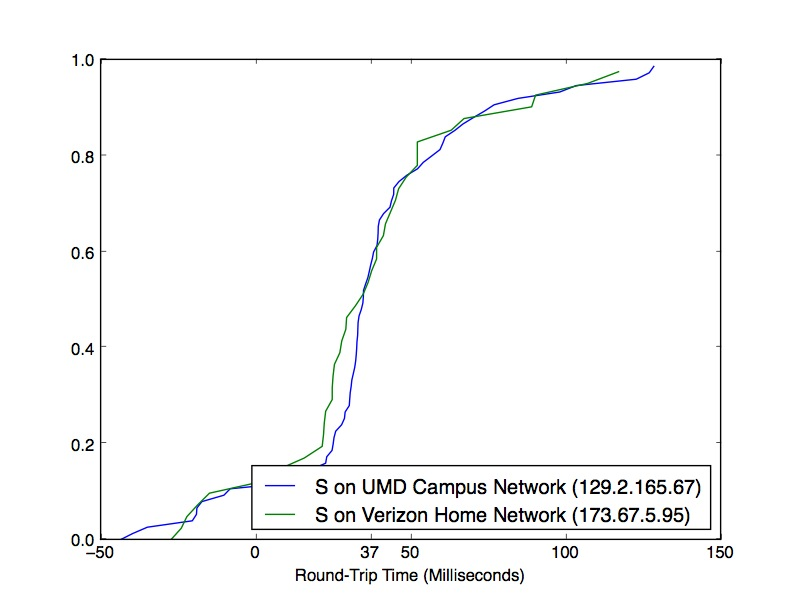
\includegraphics[width=4in]{cdf}
\caption{\label{fig:myfigure} CDF of arbitrarily changing W and Z, while leaving X and Y constant measured by host S on two different different networks.}
\end{figure*}
\section{Evaluation}

Although we eventually intend to use our tool to collect large datasets of the latencies between all relays on the Tor network, and potentially to track this information continually over time, our current study focuses on analyzing the accuracy of the data our tool collects, to first ensure that it will be reliable enough for these purposes.

We test the accuracy of our tool by constructing circuits on S (connected to the UMD campus network) in which we keep the X and Y relays constant, and randomly choose different pairs of W and Z relays. We expect that our calculated value of $R_{xy}$ should be the same for each circuit, and thus independent of any changes made to S, W Z, and D, since we cancel all of these components in the final calculation. 

In order to test this theory, we first arbitrarily select X and Y from a list of valid exit nodes to be 213.239.214.175, located in Nuremberg, Germany, and 62.149.13.57, located in Kiev, Ukraine. We then create 50 circuits on S out of these relays and two random relays, W and Z. For each of these 50 circuits, we take 10 measurements at each step of the procedure, and calculate 10 possibilities for the value of $R_{xy}$. We then consider the median of these 10 values for each circuit to be most consistently representative of the actual RTT, based on observations. Finally, we plot the cumulative distribution function of the 50 medians in Figure 2. In addition, we repeat the above trials when S is connected to a Verizon home network in Ellicott City, MD, rather than the University of Maryland campus network, and plot those results for comparison in Figure 2 as well. 

In both cases, we find that a majority of the trials center around a value of 37 milliseconds. Although we cannot directly confirm this value without controlling X and Y, the geographic distance between X and Y, about 944 miles, suggests that 37 milliseconds is reasonable. However, we also acknowledge that there are a number of outliers in this data. Considering a study conducted by Chen and Pasquale \cite{improving_path}, which found that latencies in the Tor network were highly variabile, it is likely that the variation in our calculations is a result of inconsistencies in the network, as opposed to inconsistencies in our tool. Thus, we have concluded that, although a single run of our tool may not produce a sufficiently precise value for the RTT between X and Y due to the variability of the Tor network, a series of runs over time produce a clear trend centered around a much more accurate and precise value. 

\section{Conclusion}

In this paper we have presented a novel approach for collecting latency measurements between two hosts that we do not control. Although our tool depends upon these hosts being exit relays in the Tor network, there are currently over 1,000 exit relays operating, mostly on home networks, which could still provide significant insight into home network connections. Compared to previous related work, our tool has the advantages of providing real measurements, rather than estimates, and being able to isolate the RTT between two individual hosts, as opposed to the RTT of an entire circuit. Although we found that a single run of our tool is not inherently precise due to high variability within the Tor network, we concluded that examination of a large enough sample size of runs produces a much more accurate and precise result. 

Due to the novelty of our method, there are a great number of possible directions for future work. The first is to collect a much larger sample size of RTTs for all pairs of exit nodes in the Tor network. Given the number of exit nodes currently in operation, this would require calculations for about 500,000 different pairs. While large, this could still be practically and feasibly calculated over a short time period. The next step would be to modify the method to be able to calculate RTTs between \textit{any} two relays in the Tor network. Ultimately, collecting measurements of the latency between all possible pairs of relays (over 12 million) in the network over time could provide extremely insightful data on how conditions of home networks change over time, and respond to real-world events.
 
\bibliography{biblio}
\bibliographystyle{abbrv}

\end{document}
